\section{Introduction}\label{sec:introduction}

\subsection{The Battlefield of Data}
In the modern digital landscape, data has become a highly surveilled environment where every wireless transmission leaves a trace \cite{duan2025sure}. As long as a mobile connection is maintained, a device generates a continuous stream of telemetry that forms a persistent behavioral record \cite{duan2025sure}. This footprint is captured passively by Cellular Network Operator Data Systems, which aggregate vast quantities of metadata regarding service requests, data exchanges, and handovers between tracking areas \cite{duan2025sure, duan2025moco}. Through their smartphones and the operator network infrastructure, users interact with nearby base stations for communication services such as phone calls, text messages, and Internet browsing. All of these activities are aggregated and stored in Business Support Systems (BSS) and Operating Support Systems (OSS), which serve as the foundation for operator data management \cite{duan2025sure}. Fig.~\ref{fig:data_collection} illustrates this data collection pipeline.

\begin{figure}[htbp]
\centering
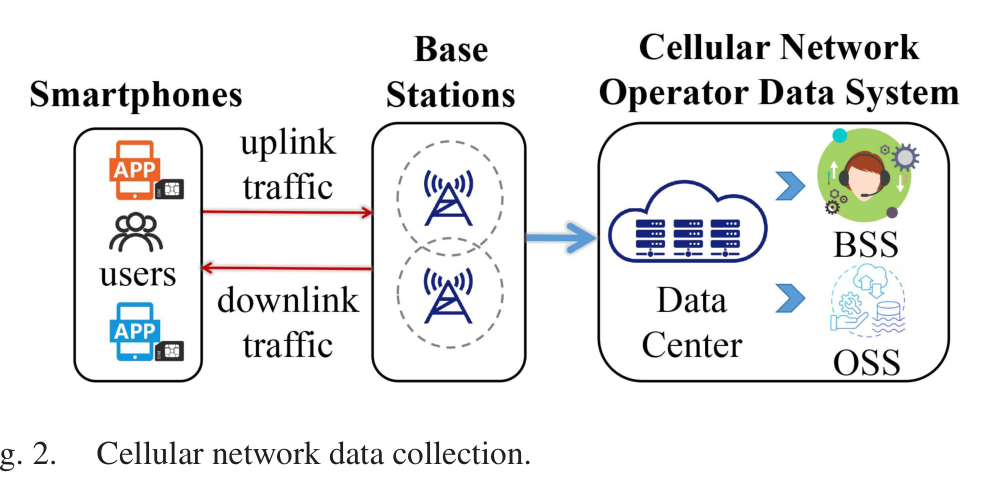
\includegraphics[width=\columnwidth]{figures/sure_fig2_data_collection.png}
\caption{Cellular network data collection pipeline: smartphones exchange uplink/downlink traffic with base stations, which forward telemetry to the operator data center for storage in BSS and OSS databases. Adapted from \cite{duan2025sure}.}
\label{fig:data_collection}
\end{figure}

\subsection{The Problem-Behavior as Identity}
The fundamental challenge is that \textbf{anonymization alone does not alter behavioral patterns} \cite{duan2025sure}. Modern forensic frameworks like SURE (Smartphone Users RE-identification) and MoCo (Mobile Contact Detection) treat behavior as identity \cite{duan2025sure, duan2025moco}. By extracting behavioral signatures from sequences of Base Station (BS) associations and traffic levels, these frameworks can uniquely identify a user \cite{duan2025sure, duan2025moco}. Research indicates that the majority of user traffic is concentrated on just two antennas the \textbf{``Top 2 BS'' rule}which serves as a spatial anchor for identifying a target's home or workplace \cite{duan2025sure}. Additionally, approximately 60\% of users exhibit consistently modest uplink traffic volumes, further enabling behavioral fingerprinting \cite{duan2025sure}.

\subsection{The Illusion of Anonymity}
Traditional security methods, such as k-anonymity and the suppression of identifiers like IMSI, are insufficient against deep learning \cite{duan2025sure, duan2025moco}. These methods fail because they only obscure identifying fields while leaving underlying spatio-temporal metadata unchanged \cite{duan2025sure, duan2025moco}. Dual-encoder architectures can mathematically bridge the gap between an anonymous index and a known identity with \textbf{AUC scores of 0.89} using only 4 days of data \cite{duan2025sure}. As shown in Fig.~\ref{fig:attack_scenario}, an adversary can leverage leaked identity data and a re-identification model to de-anonymize users from publicly shared operator datasets.

\begin{figure}[htbp]
\centering
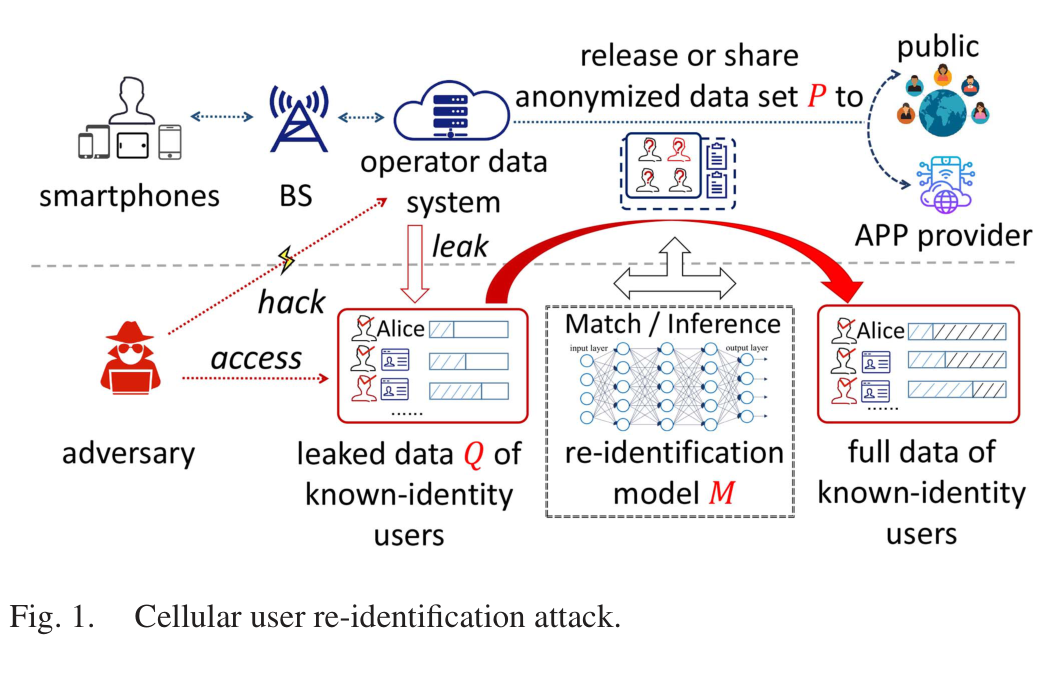
\includegraphics[width=\columnwidth]{figures/sure_fig1_attack_scenario.png}
\caption{Cellular user re-identification attack: an adversary uses leaked known-identity data $Q$ and a matching model $M$ to link anonymous records from a publicly released dataset $P$ back to real identities. Adapted from \cite{duan2025sure}.}
\label{fig:attack_scenario}
\end{figure}

\subsection{Project Objectives}
This report argues that remaining on a cellular grid creates a high re-identification risk \cite{duan2025sure, duan2025moco}. We propose \textbf{bypassing the cellular operator data system entirely} by deploying a parallel radio network built on the Meshtastic protocol \cite{meshtastic_overview}.

